\section{Background} \label{sec:background}
The dependency between the guest page table and the IOTLB is very subtle. 
To fully understand the dependency, we need to know the details about how the paravirtualized hypervisor protects itself through guest page table and IOMMU.
Specifically, we explicitly describe 1) paravirtualized MMU mode, and 2) IOMMU and DMA address translation.
As Xen~\cite{XEN-SOSP03} is a typical and popular paravirtualized hypervisor, in this section we use Xen in a x86 MMU model~\cite{x86-pv-model} to illustrate the details. We believe you can easily find the corresponding mechanisms on other paravirtualized hypervisors. 
If you are already familar with these, you can skip this section to the motivation section (Section~\ref{sec:moti}).  

%As stated above, updating page types of guest OS leads to a number of IOTLB misses, and this is related to the security policies that paravirtualized (PV) hypervisor enforces. In the PV setting, the hypervisor is responsible for protecting and updating security-sensitive data structures so as to prevent illicit accesses from guest OSes and I/O devices. 


\subsection{Paravirtualized MMU Model}\label{sec:pvmodel}
In this subsection, we first introduce the address translation machenism on x86, and then we highlight how Xen protect itself in the paravirtualized MMU model.

\subsubsection{Address Translation}\label{sec:addr-trans}
There are two steps to transform logical addresses (i.e., addresses as viewed by programmers) into physical addresses (i.e., actual addresses in physical memory): 
1) segment translation, in which a logical address (consisting of a segment selector and segment offset) are converted to a linear address, 
and 2) page translation, in which a linear address is converted to a physical address\footnote{Physical address is also called machine address in Xen setting.}.
Figure~\ref{fig:address-translation} illustrates the whole translation process.
\begin{figure}[ht]
\centering
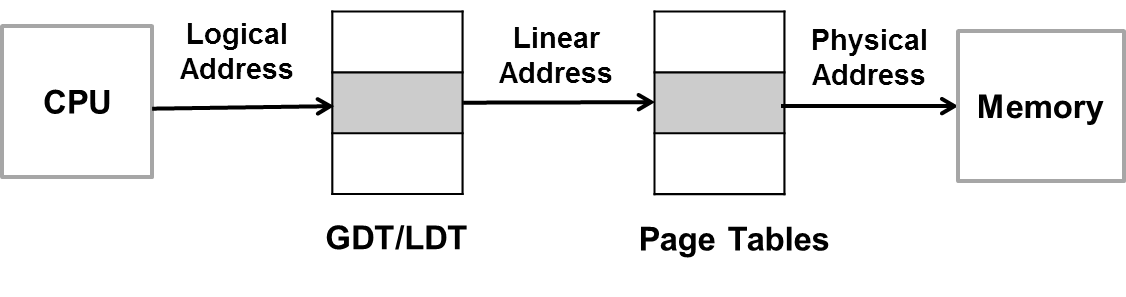
\includegraphics[width=0.5\textwidth]{image/background/address-translation.png} \\
\caption{Address Translation}
\label{fig:address-translation}
\end{figure}


\paragraph{Segementation Descriptor Table}\label{sec:gdt}
Each logical address consists of a \emph{segment} selector and an \emph{offset}, which are used to locate a segment descriptor.
A segment descriptor describes a segment, including the segment base address, limiation of the segment lenght and other meta-data.
All segment descriptors are stored in the Global Descriptor Table (GDT) or Local Descriptor Tables (LDT). 
In order to translate to the exptected linear address, the integrity of the GDT and LDT should be guaranteed. 

\paragraph{Page Table}\label{sec:pagetable}
Page tables are used by a hardware, i.e., Memory Management Unit (MMU), to translate the linear addresses into physical addresses used by the hardware to process instructions.
In the PAE-enabled paging mode, a page table has three levels: L1 level (bottom level), L2 level (middle level) and L3 level (top level).
The slots in L1, L2 and L3 levels are known as Page Table Entry (PTE), Page Middle Directory (PMD) and Page Global Directory (PGD), respectively.
A PTE slot could determine the access permissions of a page pointed by this PTE, e.g., the kernel could set a page read-only by clearing the bit within PTE slot that represents the writable permission.

There are many page tables in a guest VM, as each user process has its own page table. 
The creation and exit of a user process will be accompanied by the creation and destruction of a page table respectively.
It means that if there are numerous temporary processes generated within a period, there will be a large number of page tables created. 

\subsubsection{Page Types and Security Validations}\label{sec:pv-security}
%On the architecture of Xen, there are three layers: a hypervisor, guest OS and guest applications. 
%Unfortunately, the paging mechanism offers only two protection layers, i.e., user and supervisor spaces.
%Thus, Xen has to combine both paging and segmentation machanisms on x86. 
\begin{table}[!ht]
\begin{center}
\begin{tabular}{|p{1.7cm}|p{4.3cm}|}
\hline
{\textbf{Page Type}}  & {\textbf{Descriptions}}     \\ \hline
None & No special uses \\ \hline
L\emph{N} Page-Table Page & Pages used as a page table at level \emph{N}. There are separate types for each of the 3 levels on 32bit PAE guests. \\ \hline
Segment Descriptor Page & Pages used as part of the GDT/LDT \\ \hline
Writable Page & Pages are writable. \\ \hline
\end{tabular}
\end{center}
\caption{The page types used in Xen.}
\label{tab:pagetype}
\end{table}

In order to ensure that the guest cannot subvert the system, Xen requires that certain update policies are maintained, 
and therefore that all updates of the page tables should be vetted by Xen. 
To this end, the guest OS is deprivileged, from ring-0 to ring-1, leaving ring-0 for the Xen hypervisor.
This prevents the guest OS from executing privileged instructions, e.g., the guest OS cannot directly update control registers.

Xen also defines a number of page types, which are listed in Table~\ref{tab:pagetype}, and maintain a type count for each page.
Xen enforces the policies that any given page has exactly one type at any given time, 
and only pages with the writable type have a writable mapping in the page tables. 
By doing this it can ensure that the guest OS is not able to directly modify any page-table pages and therefore subvert the security of the system.
If the guest kernel attempts to update the page table, it has to issue a hypercall to ask the hypervisor to complete the update.
As Xen is always involved in all updaes to the page tables, the policies on the page table updates are non-bypassable.

Whenever a page table is loaded into the hardware page-table base register (cr3), 
the hypervisor must take an appropriate type reference with the L3 page-table type.
If the page is not already of the required type, then in order to take the initial reference it must first have a type count of zero.
In addition, it must be validated to ensure that it follows the following policy: 
for a page with a page-table type to be valid, it is required any pages referenced 
by a present page table entry in the page have the type of the next level down. 
For instance, any page referenced by a page with type L3 Page Table must itself have type L2 Page Table. 
This policy is applied recursively down to the L1 page table layer. 
At L1 the invariant is that any data page mapped by a writeble page table entry must have the writeable page type.
By applying these policies, Xen ensures that all page-table pages as a whole are safe to load into the page table base register.
Similar requirements are placed on other special page types, e.g., GTD/LDT pages.

The page type is allowed to be changed. 
Xen enforces that the type of a page can only be changed when the type count is zero.  
In addition, Xen also requires that every page type update is only happened between writable and non-writable pages, as summaried in Figure~\ref{fig:page-type-updates}.

\yueqiang{This figure\ref{fig:page-type-updates} should be revised. 1) font size 2) figure size and 3) rectangle is not needed to be shaded.}

\begin{figure}[ht]
\centering
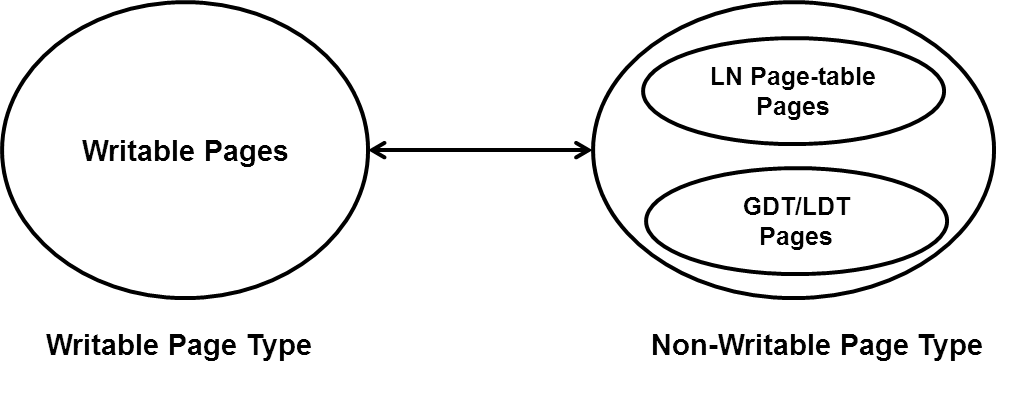
\includegraphics[width=0.45\textwidth]{image/background/page-type-updates.png} \\
\caption{Page Type Updates}
\label{fig:page-type-updates}
\end{figure}


\subsection{IOMMU and DMA address translation}
%citing: intel vt-d
The input/output memory management unit (IOMMU)~\cite{directio} is a memory management unit (MMU) that connects a DMA-capable I/O bus to the main memory. 
Like a traditional MMU, the IOMMU maps device addresses (also called as I/O addresses) to physical addresses through a dedicated page table.
This technique is also known as DMA remapping.
The IOMMU page table that is created and maintained by the hypervisor in its own space, is able to restrict the access on a particular page by configuring the permission bits.
The hypervisor grants different access permissions for different page types, such as the writable pages are always allowed full access perimissions, while the page-table pages should be always inaccessible for any device.
This is why when the page-type changes between writable page and page-table page, updating IOMMU page table is always necessary.

However, the DMA remapping is always need the page table walking, which is slow and inefficient. 
To accelarate the translation speed, the I/O translation look-aside buffer (IOTLB) is introduced. 
The IOTLB is to cache frequently accessed page table entries. 
By doing so, the IOTLB is very likely to occur, meaning the physical address of a queried DMA address will be immediately fetched through the IOTLB path (Figure~\ref{fig:subfig:a}).
If unlikely the IOTLB miss occurs, the DMA remapping still can go the slow page-table path to get the physical address (Figure~\ref{fig:subfig:b}). 
To achieve a better I/O performance, the DMA remapping should avoid take the page-table path frequently.

\begin{figure}
\centering
\subfigure[IOTLB Path]{
\label{fig:subfig:a}

\includegraphics[width=0.5\textwidth]{image/background/DMA-IOTLB-translation.png}}
\hspace{1in}
\subfigure[Page-Table Path]{
\label{fig:subfig:b}
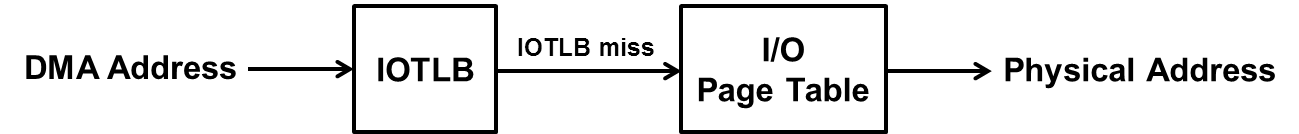
\includegraphics[width=0.5\textwidth]{image/background/DMA-pt-translation.png}}
\caption{DMA Address Translation}
\label{fig:dma-add-trans} %% label for entire figure
\end{figure}

%talking about how to flush IOTLB
%invalidation requests and invalidation interface
According to IOMMU speficiation~\cite{intelvt}, a typical IOMMU is able to provide three types of IOTLB invalidation schemes, i.e., global invalidation, domain-selective invalidation, page-selective invalidation, which differ in granularity. 
Specifically, the golbal invalidation will always invalidate all IOTLB entries as a whole.
The domain-selective invalidation only invalidates the selected VM domain's IOTLBs, whose performance is a little better than the previous golbal invalidation.
The page-selective invalidation that only invalidate the corresponding IOTLB could achieve the best performance, comparing with the previous two schemes.
%Intuitively, when a requested entry that corresponds to a specified DMA address needs to be invalidated, a page-selective invalidation is the best choice for the sake of performance. 
Besides the invalidation scheme, IOMMU also supports two kinds of invalidation interfaces: register based invalidation and queued invalidation interface, between which queued invalidation performs better.
No matter the IOTLB flushes frequently in whatever granularity, it will inevitably increases the probability of IOTLB misses, thereby introduce negative effects on the I/O performance. 
%And this is where our motivation lies.
